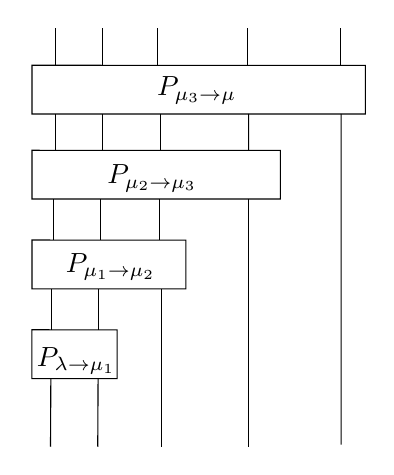
\begin{tikzpicture}[yscale=-1,scale=0.03,baseline={([yshift=-.5ex]current bounding box.center)}]
\begin{scope}[shift={(0.00mm,719.29mm)}]
% path id='path4807'
% path spec='m 142.85714,-562.4137 0,206.2045 1411.42856,0 0,-205.71429 z'
\draw [fill=none,draw=black] (142.86mm,-562.41mm)
-- ++(0.00mm,206.20mm)
-- ++(1411.43mm,0.00mm)
-- ++(0.00mm,-205.71mm)
-- cycle
;
% path id='path4809'
% path spec='m 142.78887,-202.48199 0,206.3410633 1051.56513,0 0,-205.8505233 z'
\draw [fill=none,draw=black] (142.79mm,-202.48mm)
-- ++(0.00mm,206.34mm)
-- ++(1051.57mm,0.00mm)
-- ++(0.00mm,-205.85mm)
-- cycle
;
% path id='path4811'
% path spec='m 142.69719,177.42629 0,206.52447 651.74854,0 0,-206.03349 z'
\draw [fill=none,draw=black] (142.70mm,177.43mm)
-- ++(0.00mm,206.52mm)
-- ++(651.75mm,0.00mm)
-- ++(0.00mm,-206.03mm)
-- cycle
;
% path id='path4813'
% path spec='m 142.61017,557.33924 0,206.69857 360.49405,0 0,-206.20718 z'
\draw [fill=none,draw=black] (142.61mm,557.34mm)
-- ++(0.00mm,206.70mm)
-- ++(360.49mm,0.00mm)
-- ++(0.00mm,-206.21mm)
-- cycle
;
% path id='path4815'
% path spec='m 1448.5714,-561.92349 0,-157.14285'
\draw [fill=none,draw=black] (1448.57mm,-561.92mm)
-- ++(0.00mm,-157.14mm)
;
% path id='path4819'
% path spec='m 1451.7857,-356.56635 -0.3571,1400.35715'
\draw [fill=none,draw=black] (1451.79mm,-356.57mm)
-- ++(-0.36mm,1400.36mm)
;
% path id='path4821'
% path spec='m 1054,-719.26278 0,156.98376'
\draw [fill=none,draw=black] (1054.00mm,-719.26mm)
-- ++(0.00mm,156.98mm)
;
% path id='path4825'
% path spec='m 1059.8906,-356.6087 0.062,154.73139'
\draw [fill=none,draw=black] (1059.89mm,-356.61mm)
-- ++(0.06mm,154.73mm)
;
% path id='path4827'
% path spec='m 1060.5,3.36222 0,1048.84888'
\draw [fill=none,draw=black] (1060.50mm,3.36mm)
-- ++(0.00mm,1048.85mm)
;
% path id='path4848'
% path spec='m 676,-718.85098 0,156.20457'
\draw [fill=none,draw=black] (676.00mm,-718.85mm)
-- ++(0.00mm,156.20mm)
;
% path id='path4852'
% path spec='m 686,-356.2756 0,153.7297'
\draw [fill=none,draw=black] (686.00mm,-356.28mm)
-- ++(0.00mm,153.73mm)
;
% path id='path4854'
% path spec='m 684,3.956632 0,173.750518'
\draw [fill=none,draw=black] (684.00mm,3.96mm)
-- ++(0.00mm,173.75mm)
;
% path id='path4856'
% path spec='m 692,383.86226 0,668.50004'
\draw [fill=none,draw=black] (692.00mm,383.86mm)
-- ++(0.00mm,668.50mm)
;
% path id='path4858'
% path spec='m 422.6417,764.12246 -1.41421,288.39914'
\draw [fill=none,draw=black] (422.64mm,764.12mm)
-- ++(-1.41mm,288.40mm)
;
% path id='path4860'
% path spec='m 425.28263,383.81666 0,174.02973'
\draw [fill=none,draw=black] (425.28mm,383.82mm)
-- ++(0.00mm,174.03mm)
;
% path id='path4862'
% path spec='m 432.5412,3.8112543 0,173.7714857'
\draw [fill=none,draw=black] (432.54mm,3.81mm)
-- ++(0.00mm,173.77mm)
;
% path id='path4864'
% path spec='m 441.02648,-356.28287 0,153.70733'
\draw [fill=none,draw=black] (441.03mm,-356.28mm)
-- ++(0.00mm,153.71mm)
;
% path id='path4866'
% path spec='m 442.44069,-719.20542 0,156.71253'
\draw [fill=none,draw=black] (442.44mm,-719.21mm)
-- ++(0.00mm,156.71mm)
;
\node [black] at (840.00mm,-455.64mm) { $P_{\mu_3 \to \mu}$ };
\node [black] at (652.00mm,-83.64mm) { $P_{\mu_2 \to \mu_3}$ };
\node [black] at (476.00mm,292.36mm) { $P_{\mu_1 \to \mu_2}$ };
\node [black] at (330mm,688.36mm) { $P_{\lambda \to \mu_1}$ };
% path id='path4236'
% path spec='m 222.6417,764.12246 -1.41421,288.39914'
\draw [fill=none,draw=black] (222.64mm,764.12mm)
-- ++(-1.41mm,288.40mm)
;
% path id='path4238'
% path spec='m 225.28263,383.81666 0,174.02973'
\draw [fill=none,draw=black] (225.28mm,383.82mm)
-- ++(0.00mm,174.03mm)
;
% path id='path4240'
% path spec='m 232.5412,3.8112543 0,173.7714857'
\draw [fill=none,draw=black] (232.54mm,3.81mm)
-- ++(0.00mm,173.77mm)
;
% path id='path4242'
% path spec='m 241.02648,-356.28287 0,153.70733'
\draw [fill=none,draw=black] (241.03mm,-356.28mm)
-- ++(0.00mm,153.71mm)
;
% path id='path4244'
% path spec='m 242.44069,-719.20542 0,156.71253'
\draw [fill=none,draw=black] (242.44mm,-719.21mm)
-- ++(0.00mm,156.71mm)
;
\end{scope}
\end{tikzpicture}
